\documentclass[12pt,a4paper]{article}

\usepackage[portuguese]{babel}
\usepackage{hyperref} % fazer direcionamento das referências
\usepackage{graphicx} % pacote para figuras

% Cabeçalho
\title{Latex e R Sweave} % titulo
\author{Larissa Tavares} % autor

\usepackage{Sweave}
\begin{document}
\Sconcordance{concordance:page.tex:page.Rnw:%
1 10 1 1 0 182 1 1 2 1 0 1 1 7 0 1 2 2 1 1 3 5 0 1 2 2 1 1 2 1 0 2 1 4 %
0 1 2 2 1 1 2 1 0 2 1 4 0 1 2 5 1 1 2 1 0 2 1 4 0 1 2 6 1 1 2 1 0 1 1 1 %
4 7 0 1 2 4 1 1 2 1 0 2 1 10 0 1 2 17 1}


\maketitle % comando para mostrar o título e autor

% colocar o índice e listas de tabela
\tableofcontents % indice
\listoffigures % lista de figuras
\listoftables % lista de tabelas

%\chapter{Introdução}

\section{O que é o RLadies ?} % criando seção dentro do capítulo

O R-Ladies é uma iniciativa de impacto social que foca em ensinar a linguagem estatística (R) para mulheres cis e público LGBTQIA+ que não têm recursos e/ou oportunidades para aprender a programar.

\subsection{Qual a missão do RLadies?}

Apoiar grupos minoritários para que alcancem seu potencial de programação na linguagem R.

Construímos uma rede global colaborativa de líderes, mentores, aprendizes e desenvolvedoras para facilitar o progresso individual e coletivo em todo o mundo.

\section{Exemplos de aplicação}

\textit{Teste italico}

\textbf{Teste em negrito}

\underline{sublinhado}

\textit{\textbf{Italico e negrito}}

\textit{\textbf{\underline{Italico,sublinhado e negrito}}}

\newpage

\subsection{Nota de rodapé}

Exemplo para uma nota de rodapé \footnote{Nota de rodapé}.

\section{Fórmulas}

50\% das pessoas

Basta colocar as equações entre \textbf{\$}.

$X = y + 1$
  
  Temos vários argumentos para deixar as equações mais sofisticadas. Temos comandos para frações, símbolos e etc. Quando usamos um \textbf{\$} a fórmula fica no canto esquerdo ou no meio do texto, utilizando dois \textbf{\$} a fórmula fica centralizada na página.

Teste um apenas um \$ : 
  $Z = \frac{x}{y}$
\newline
  
  Teste de fórmula centralizada :
  $$W = \theta * \alpha$$
  
  Podemos definir fórmulas de outra maneira, usando o comando \textit{equation}. Desta forma podemos enumerar as equações e cita-las no texto. É útil em livros e trabalhos acadêmicos. Vamos observar a Equação \ref{formula}.

\begin{equation}
W = \sum_{i=1}^{n} = \theta * \alpha
\label{formula}
\end{equation}

\section{Criando Tabelas}

A seguir temos a Tabela \ref{Tab:Tcr}, nela encontramos um exemplo de tabela com duas colunas e 3 linhas. Vamos mostrar alguns tipos de tabelas, a primeira é apenas a tabela, sem demarcar as linhas e colunas.

\begin{table}
\caption{Exemplo de tabelas}
\begin{tabular}{lllll}
Marina & Ponto &  \\
1      & 5     &  \\
2      & 7     &  \\
3      & 8    
\end{tabular}
\label{Tab:Tcr}
\end{table} 

Agora vamos mostrar o exemplo de uma tabela onde demarcamos linhas nas linhas e colunas. Vamos observar a Tabela \ref{tab:exemplo}.


\begin{table}[!h]
\centering
\caption{Exemplo de tabelas 2}
\label{tab:exemplo}
\begin{tabular}{|l|l|}
\hline
Marina & Ponto \\ \hline
1      & 5     \\ \hline
2      & 7     \\ \hline
3      & 8     \\ \hline
\end{tabular}
\end{table}

O comanhdo \textit{centering} é para centralizar a tabela no texto. Se preferir, pode deixar a tabela no canto esquerdo da página, basta retirar o comando.

\begin{table}[!h]
\caption{Exemplo de tabelas 3}
\label{tab:exemplo2}
\begin{tabular}{|l|l|}
\hline
Marina & Ponto \\ \hline
1      & 5     \\ \hline
2      & 7     \\ \hline
3      & 8     \\ \hline
\end{tabular}
\end{table}

Podemos também mudar a legenda da tabela, ela pode ficar na parte superior da tabela ou na parte inferior, basta colocar o comando \textit{caption} na ordem que deseja.

\begin{table}[!h]
\centering
\begin{tabular}{|l|l|}
\hline
Marina & Ponto  \\ \hline
1      & 5      \\ \hline
2      & 7      \\ \hline
3      & 8   \\ \hline
  \hline
\end{tabular}
\caption{Exemplo de tabela sem centralização}
\label{tab:ex2}
\end{table}


\section{Criando Figuras}
Para acrescentar uma figura/imagem no seu texto, você precisa que o arquivo esteja na mesma pasta que o seu texto. A imagem pode ser em vários formatos diferentes. Vamos observar um exemplo na Figura \ref{fig:teste}

\begin{figure}[h!]
\centering

\includegraphics[width=0.4\textwidth]{bolinho.png}
\caption{Título da figura}
\label{fig:teste}
\end{figure}

Para mudar a posição da legenda, é a mesma ideia das tabelas, usando o comando \textit{caption}. Vamos colocar a legenda na parte superior da imagem.

\begin{figure}[!]
\centering
\caption{Título da figura - Legenda em cima}
\label{fig:teste2}

\includegraphics[width=0.4\textwidth]{bolinho.png}
\end{figure}


\newpage

\section{Criando listas}

Podemos listar os itens com o marcador de pontos.  

\begin{itemize}
\item R
\item Rstudio
\item R Sweave
\item R Ladies
\end{itemize}

Outra forma é criar uma lista enumerada. 
\begin{enumerate}
\item R
\item Rstudio
\item R Sweave
\item R Ladies
\end{enumerate}

\subsection{Usando citações}

\begin{itemize}
\item \textbf{Exemplo: } Os comandos básicos de R foram inseridos segundo \cite{ref1}. 
\item \textbf{Exemplo 2:} Utilizaremos o RStudio para fazer as análises \cite{rstudio}
\item \textbf{Exemplo 3:} Utilizando mais de uma referência. Uma para o Sweave e outra para o Triola \cite{sweave, triola}
\end{itemize}

\newpage % pular uma página

\section{R e Latex}

Vamos agora apresentar alguns exemplos de códigos no meio do texto, assim você pode plotar os gráficos, exibir tabelas e apresentar as suas análises. Podemos juntar tudo em apenas uma ferramenta. 

Podemos usar as bases de dados disponíveis no R, como por exemplo a base de dados \textbf{Iris}, essa é uma base de dados sobre flores de 3 espécies.

\begin{Schunk}
\begin{Sinput}
> data(iris)
> summary(iris$Species)
\end{Sinput}
\begin{Soutput}
    setosa versicolor  virginica 
        50         50         50 
\end{Soutput}
\end{Schunk}

Para mostrar apenas os resultados sem o comando, basta acrescentar os argumentos no chunk.

\begin{Schunk}
\begin{Soutput}
    setosa versicolor  virginica 
        50         50         50 
\end{Soutput}
\end{Schunk}

Podemos gerar valores, fazer operações e pedir para imprimir os resultados. 

\begin{Schunk}
\begin{Sinput}
> set.seed(0205) # fixando semente
> x = rnorm(100,1,10)
> hist(x)
\end{Sinput}
\end{Schunk}
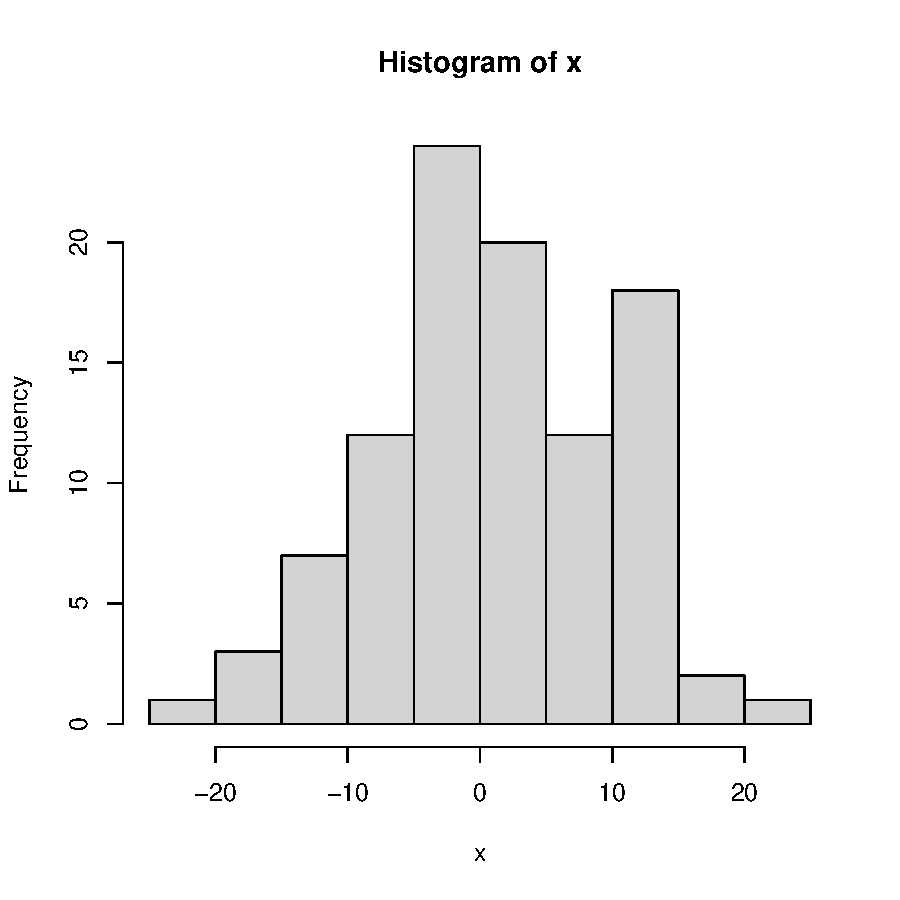
\includegraphics{page-003}

Podemos escolher também o tamanho da figura.

\begin{Schunk}
\begin{Sinput}
> set.seed(0205) # fixando semente
> x = rnorm(100,1,10)
> hist(x, col="lightblue")
\end{Sinput}
\end{Schunk}
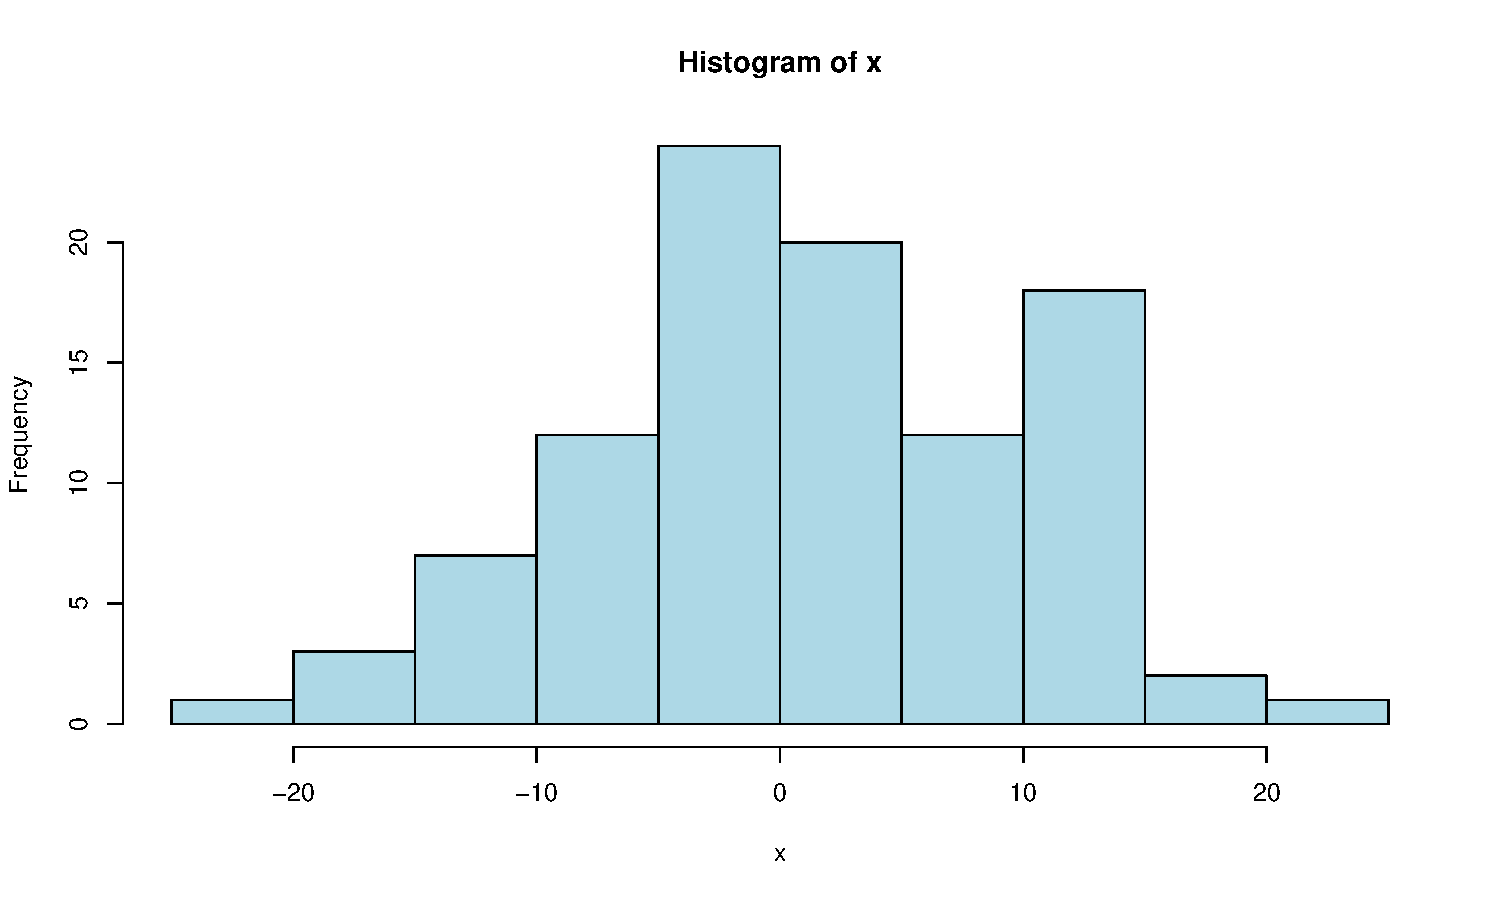
\includegraphics{page-004}

Para colocar legenda e dar uma "label" para a sua imagem, basta usar os comandos das figuras. 

\begin{figure}[!h]
\centering

\begin{Schunk}
\begin{Sinput}
> set.seed(0205) # fixando semente
> x = rnorm(100,1,10)
> hist(x, col="lightblue")
\end{Sinput}
\end{Schunk}
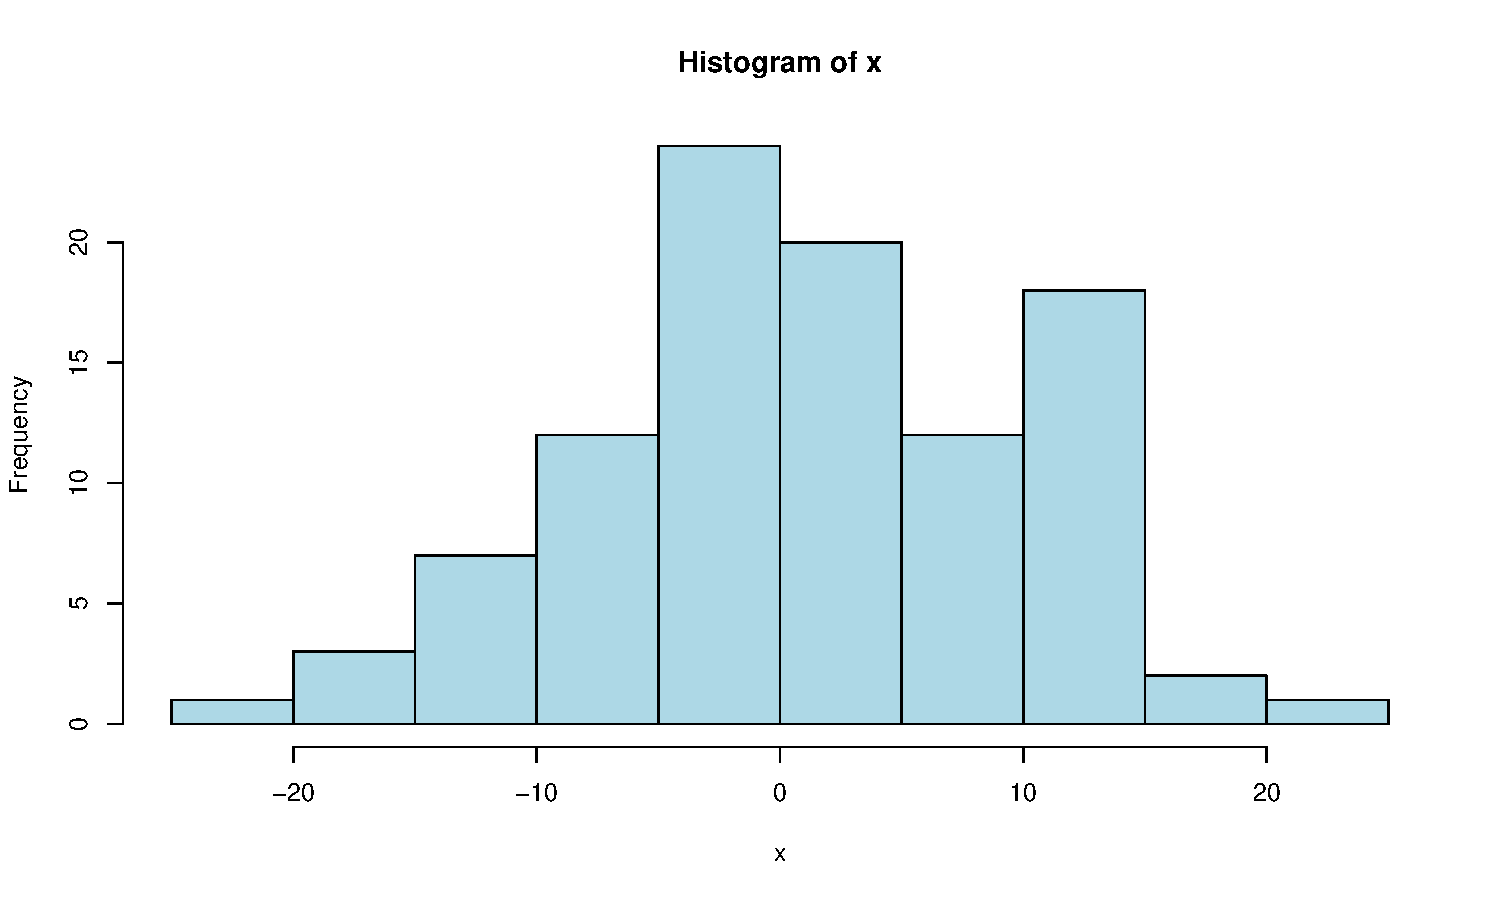
\includegraphics{page-005}

\caption{Gráfico gerado no R}
\label{fig:graf}
\end{figure}

Podemos usar os pacotes normalmente. Lembrando que se é a primeira vez que esta usando o pacote você deve instalar ele na máguina ou no RStudio cloud.

\begin{Schunk}
\begin{Sinput}
> data(iris)
> require(ggplot2)
> ggplot(data=iris, aes(x= Species, y=Sepal.Length, fill=Species))+
+   geom_bar(stat="identity")+
+   theme_minimal()+
+   scale_y_continuous(breaks=seq(0,300,20))
\end{Sinput}
\end{Schunk}
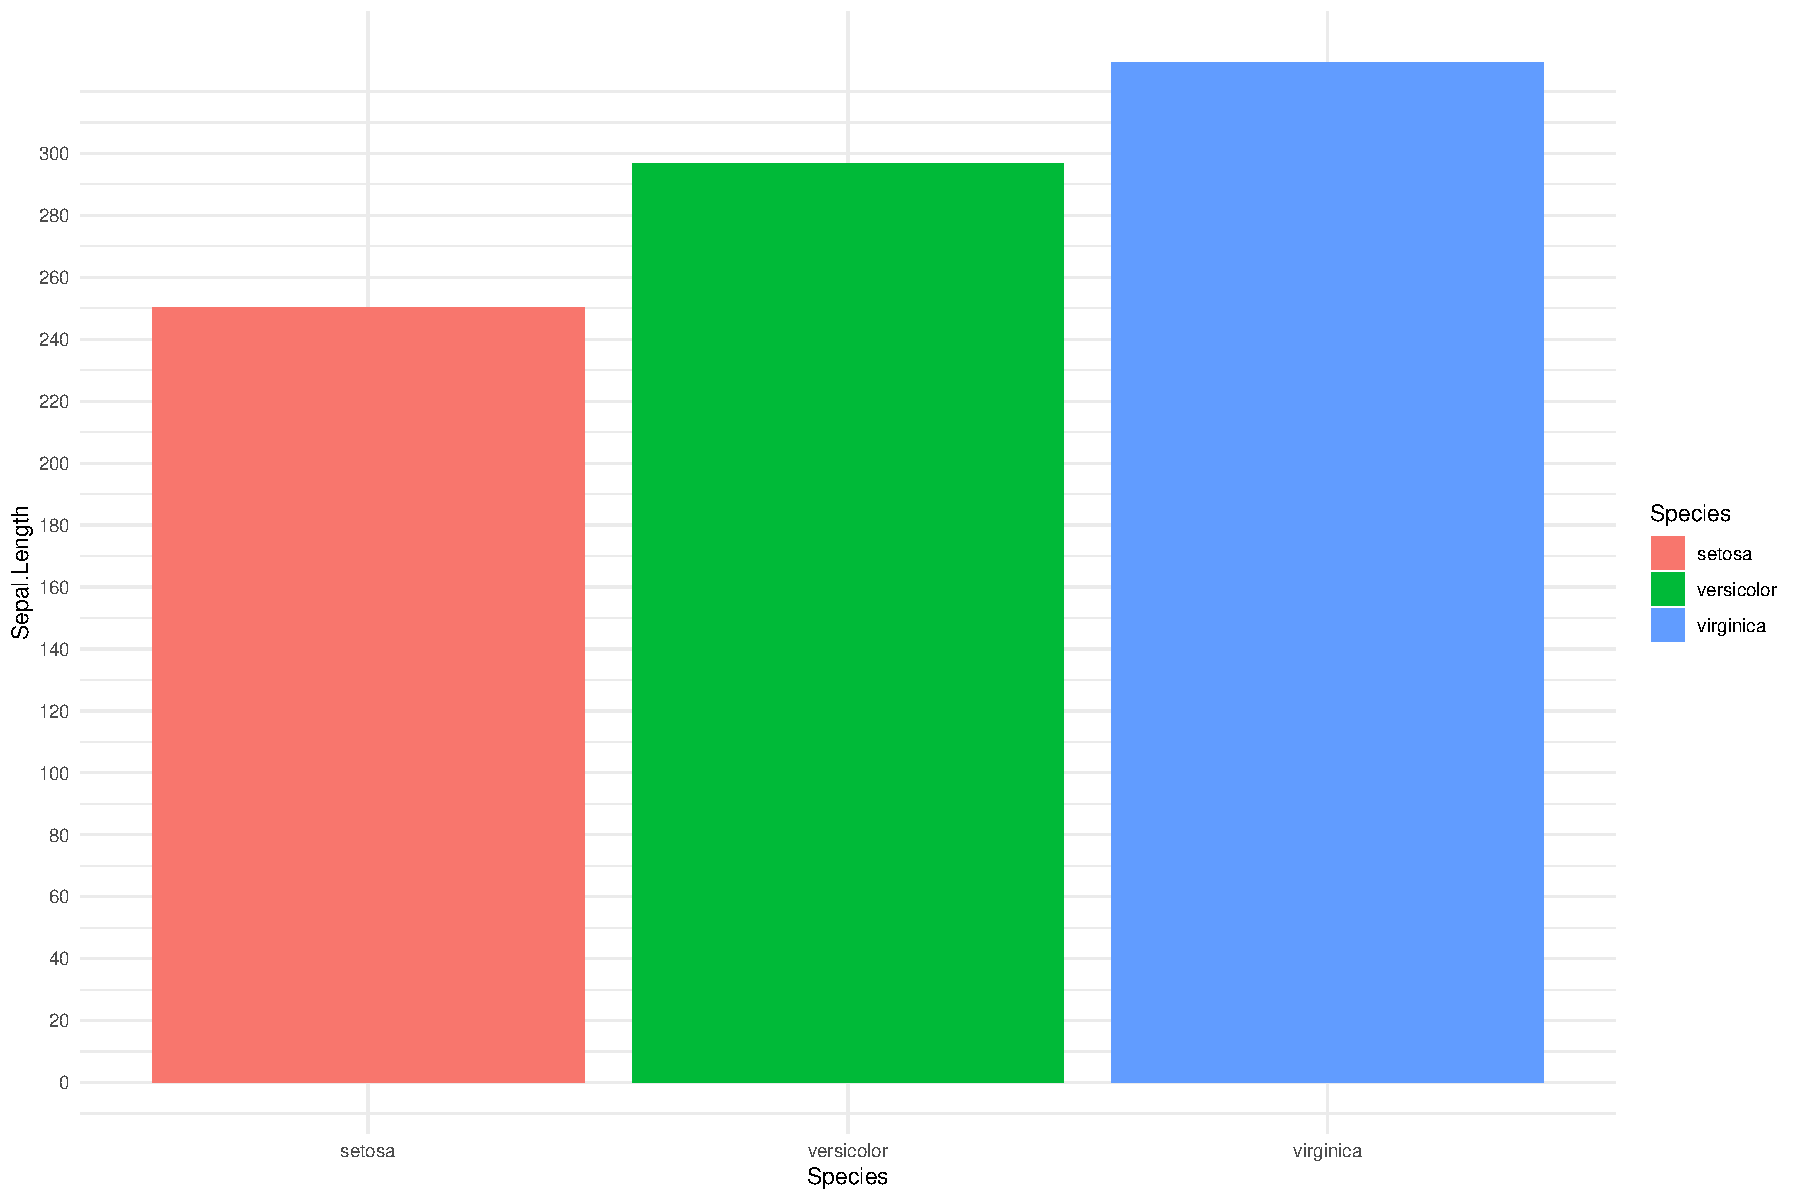
\includegraphics{page-006}

se quiser omitir o código basta acrescentar o comando \textbf{echo=FALSE} no cabeçalho do chunk.

Podemos costumisar as saídas, um exemplo é a tabela. No documento do pacote knitr tem várias opções de tabelas.

\begin{Schunk}
\begin{Sinput}
> require(knitr)
> require(dplyr)
> table(iris$Species) %>% kable(col.names = c("Espécie", "Frequência"))
\end{Sinput}
\begin{Soutput}
|Espécie    | Frequência|
|:----------|----------:|
|setosa     |         50|
|versicolor |         50|
|virginica  |         50|
\end{Soutput}
\end{Schunk}


\newpage % pular uma página


%\bibliographystyle{unsrt}
\bibliographystyle{apalike}  

\bibliography{bibliografia.bib} % arquivo .bib


\appendix{}

\section{Anexo}

A comunidade R-Ladies é uma organização sem fins lucrativos que promove a diversidade de gênero na comunidade da linguagem computacional estatística R. Contamos atualmente com pouco mais de 130 grupos espalhados em 44 países, com aproximadamente mais de 35000 pessoas participando ativamente da comunidade. Veja mais aqui: R-Ladies Global \url{https://rladiesbh.com.br}

\end{document}
